%% LaTeX2e class for student theses
%% sections/content.tex
%% 
%% Karlsruhe Institute of Technology
%% Institute for Program Structures and Data Organization
%% Chair for Software Design and Quality (SDQ)
%%
%% Dr.-Ing. Erik Burger
%% burger@kit.edu
%%
%% Version 1.3.5, 2020-06-26

\chapter{Introduction}
\label{ch:Introduction}

%% -------------------
%% | Example content |
%% -------------------

Metal Catalysts are crucial to a variety of applications, from water splitting to CO2 reduction.
% TODO: Elaborate
The metal catalysts used used here are constructed by combining different structures around a central Iridium atom.
This allows for quick generation of thousands of different catalyst molecules.
For all catalysts in the dataset the activation barrier, along with other properties, is then computed.
Overall, a total of 1947 species with different structures are constructed.
\\
Intuitively no rule for the activation barrier can be found. Seemingly small changes in the catalysts shape can have 
a large influence on the catalysts activation barrier.
\\
Computing this activation barrier is highly complex and therefor very costly. 
Also by just computing the activation barrier, no intuition about which parts of the catalyst contribute to increasing or decreasing the activation barrier can learned.
This intuition however is required if the molecular structure should be adapted later to increase or decrease the activation barrier.
\\
The seemingly arbitrary nature in combination with requiring intuition about the origin of the activation barrier is 
reason to use neural network based regression methods.
Neural networks have become the go-to method for high dimensional regression and classification for their ability to adapt well to complex data.
\\
A limitation of neural networks however is their fixed-size input space.
Therefor a representation of the catalyst needs to be found that encodes our molecule into a fixed-size set of features.
These features will then be fed into our neural network for training. 
\\
In previous works, multiple different techniques are proposed to extract features from a catalyst molecule \cite{friederich_dos}.
While these techniques are based on the chemical structure of a molecule, they do not take into account its 3D spacial structure.
The feature extracting methods developed in this bachelor thesis will rely heavily on the 3D structure of molecule.
The idea being that the 3D structure plays an important role in the activation barrier, and encoding the 3D structure will enhance regression accuracy.
Additionally encoding the 3D structure will allow to learn about the space surrounding the central 
Iridium atom to understand the importance of location of the atoms in our molecule.
\\

3D structural encoding however comes with its own set of challenges. 
One more general being neural networks sensitivity to rotation and positioning.
Since a molecules activation barrier does not change depending on its rotation or location in space, 
information about rotation and translation should ideally not be part of the molecules features.
\\
In the case of the metal catalysts, achieving translational invariance is trivial.
Since every catalyst is constructed around exactly one metal atom, the molecule can be centered around this metal atom.

For rotational invariance the problem is more complex.
Every catalyst has a reaction pocket attached to it's cental atom.
This reaction pocket has a fixed position.
With the vector from the center of the Iridium atom to the center of the reaction pocket, two more degrees of freedom can be removed.
For the last degree of freedom, rotations around this vector, there is no natural way to get rid of it.

Here, 2 different approaches to this last degree of freedom are explored.
The first is a rotationally invariant description using fourier coefficients.

The second is using data augmentation to teach the neural network about all possible rotations.
This means the molecule is rotated along the last remaining axis of freedom, and and multiple examples of the same molecule at different rotations are used as training examples for the neural network.
This ideally allows the network to learn the molecules structure independent of it's rotation.


\section{Dataset}

The dataset contains 1947 examples of catalyst molecules.
For each atom of the molecule, the location in space is given.
For each molecule it's activation barrier is known.

The molecules were generated by combining ligands around a central Iridium atom as illustrated in \autoref{fig:chemspace}.
The activation barrier was then calculated.
Due to this combinatorial approach the dataset could later be increased with relatively low effort.
Together this gives a dataset containing the structure and the associated activation barrier for 1947 Iridium catalysts.

When examining the dataset by hand, the connection between a molecules structure and it's activation barrier is not obvious.
Seemingly small changes can have a big influence on it's activation barrier.
% TODO: Add example
A rule to guess the activation barrier from the molecules structure can not easily be found.

\begin{figure}
  \centering
  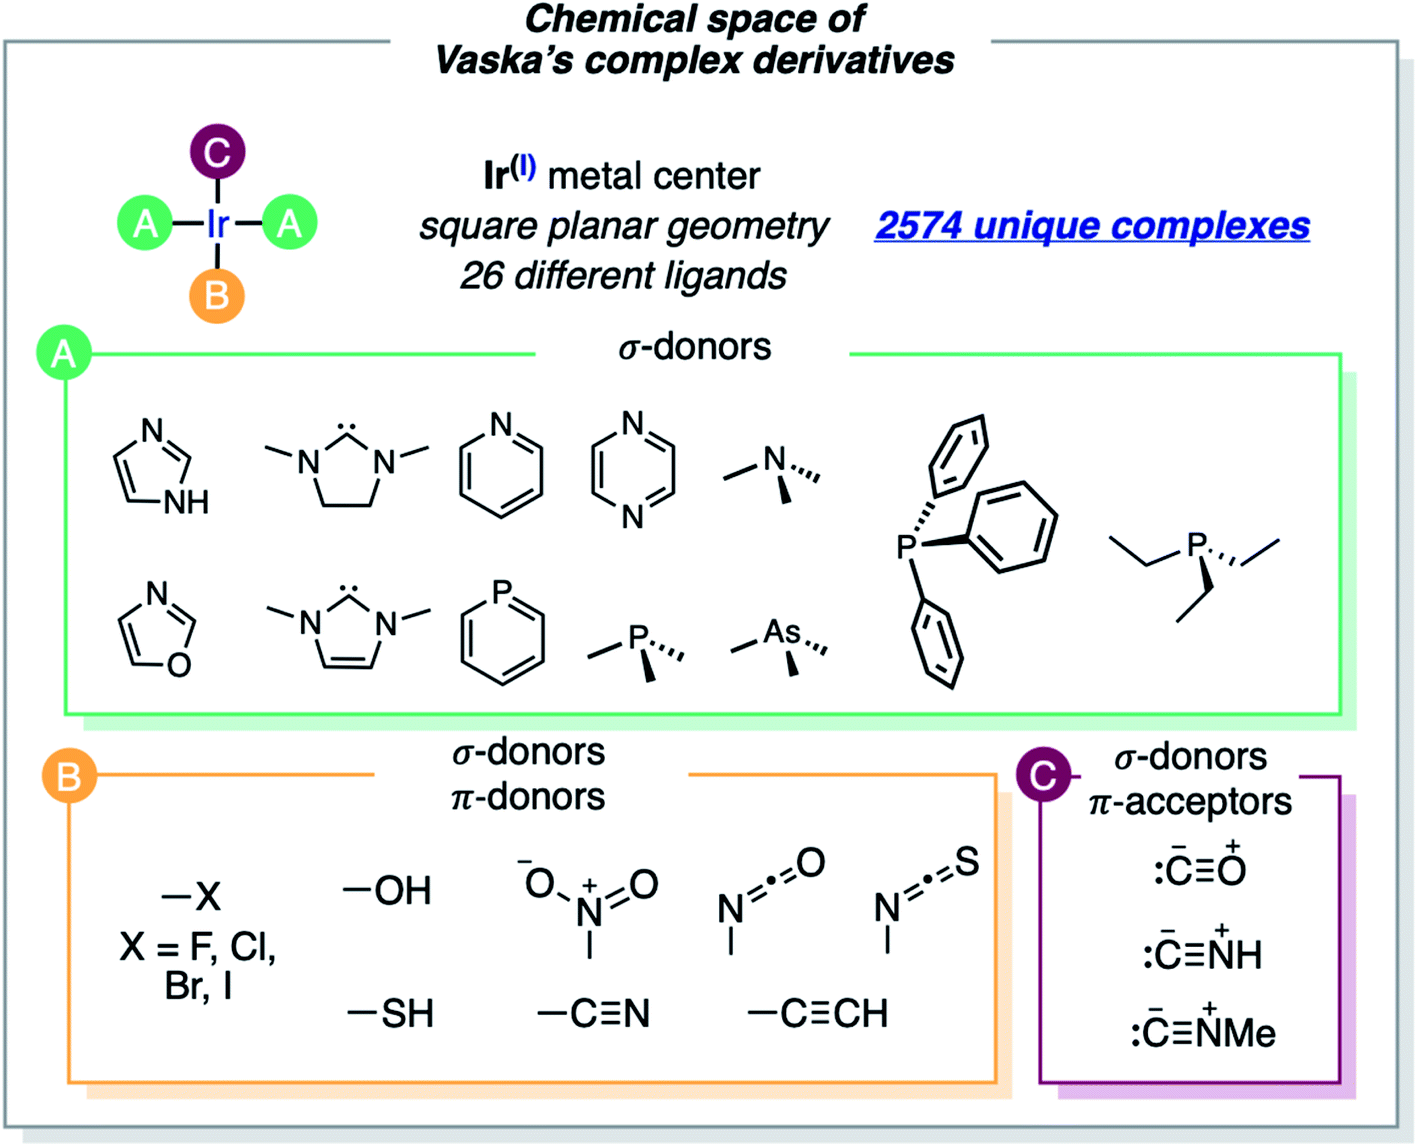
\includegraphics[width=10cm]{figures/introduction/chem-space.png}
  \caption{Ligands defining the chemical space associated with Vaska's complex. Reprinted from \cite{friederich_dos}.}
  \label{fig:chemspace}
\end{figure}
  

\section{Previous research}

In previous approaches different machine learning methods were used to predict the activation barrier of elements.
However, the features extracted from the molecule did not take into account the spacial structure of the element.
The elements were instead encoded by creating a graph from the chemical structure.
The elements are then grouped by their distance from the metal center.
For each group of elements, different features are computed as sum of pairwise products/differences of their atomic properties(such as electronegativity, atomic number, identity, topology and size) \cite{friederich_dos}.
Note that these features do not contain any information about the 3D location of the atoms.

Using these autocorrelation features, a neural network and gaussian processes and other forms of regression were used to predict the activation barrier.
Neural networks and gaussian processes both were able to predict the activation barrier within an error of $<1 kcal/mol$ for a test split of $10\%$

Other than the obvious disadvantage of not encoding location information, another disadvantage is the lack of interpretability of results.
While these features succeed at predicting reaction barriers, information what part of the molecule is contributing to the prediction is limited.

The feature extractors introduced in this thesis aim to solve this problem by extracting features that allow for a
partly reconstruction of the chemical space and thus knowing which region of the molecule contributes to a prediction.


\section{Objectives}



\section{Example: Figures}
\label{sec:Introduction:Figures}
\begin{figure}
\centering

\includegraphics[width=4cm]{logos/sdqlogo}
\caption{SDQ logo}
\label{fig:sdqlogo}
\end{figure}

A reference: The SDQ logo is displayed in \autoref{fig:sdqlogo}. 
(Use \code{\textbackslash autoref\{\}} for easy referencing.) 

\section{Example: Tables}
The \texttt{booktabs} package offers nicely typeset tables, as in \autoref{tab:atable}.

\label{sec:Introduction:Tables}
\begin{table}
\centering
\begin{tabular}{r l}
\toprule
abc & def\\
ghi & jkl\\
\midrule
123 & 456\\
789 & 0AB\\
\bottomrule
\end{tabular}
\caption{A table}
\label{tab:atable}
\end{table}

\section{Example: Formula}
One of the nice things about the Linux Libertine font is that it comes with
a math mode package.
\begin{displaymath}
f(x)=\Omega(g(x))\ (x\rightarrow\infty)\;\Leftrightarrow\;
\limsup_{x \to \infty} \left|\frac{f(x)}{g(x)}\right|> 0
\end{displaymath}

%% --------------------
%% | /Example content |
%% --------------------